%Dies ist die Hauptseite des Dokumentes. Es werden u. a. alle Kapitel,
%Einstellung im Header eingebunden.  Veränderungen müssen in folgenden Dateien
%vorgenommen werden:
      %- einzelne Kapitel (evtl. erweitern)

% Declare document wide classes
\documentclass[
    11pt,                   % Default font size
  DIV12,
    oneside,                % One-sided document
    titlepage,              % Has a specific page for the title
    parskip=half,           % Spacing between paragraphs
    headings=normal,        % Smaller headings size
    captions=tableheading,
    final                   % Document is marked as final
]{scrreprt}               %

% Include the packages
% Do we need this?
\usepackage{fix-cm}

\usepackage{amssymb} % For checkmark/cross symbols


% Do we need this?
\usepackage[T1]{fontenc}
\usepackage{lmodern}
\usepackage[utf8]{inputenc}

% Setting language of babel to english
\usepackage[english]{babel}

% Helpers for geometry and spacing settings
\usepackage{geometry}
\usepackage{setspace}

% Adapt font sizes for different sections
\usepackage{relsize}

% Lines in header and footer
\usepackage[headsepline, footsepline, ilines]{scrlayer-scrpage}

% Graphics and colors
\usepackage{xcolor}
\usepackage{graphicx}

% Hyphenation and underlining
\usepackage{soul}

% Additional font family
\usepackage{helvet}

% Big tables
\usepackage{longtable}
\usepackage{array}
\usepackage{ragged2e}
\usepackage{lscape}

\usepackage{enumitem}

% Options for pdf generation
\usepackage[
  bookmarks,
  bookmarksopen=true,
  colorlinks=true,
  linkcolor=black,        % Links have black color
  anchorcolor=black,      % Links have black color
  citecolor=black,        % Links have black color
  filecolor=black,        % Links have black color
  menucolor=black,        % Links have black color
  urlcolor=black,         % Links have black color
  backref,                % Do we need this?
  pagebackref,            % Do we need this?
  plainpages=false,       % Allows setting bookmarks (Do we need ths?)
  pdfpagelabels,          % Allows setting bookmarks (Do we need ths?)
  hypertexnames=false,    % Allows setting bookmarks (Do we need ths?)
  linktocpage             % Link page numbers in table of contents
  ]{hyperref}

  \usepackage{verbatim}

\usepackage{svg}






% Geometric specific settings
\geometry{
    paper=a4paper,
    top=25mm,
    left=25mm,
    right=25mm,
    bottom=45mm,
    pdftex
  }

% Page layout
\onehalfspace        % 1.5x spacing

\pagestyle{scrheadings}

% Header and footer on new section pages
\renewcommand*{\chapterpagestyle}{scrheadings}

% Font size of headers
\renewcommand{\headfont}{\normalfont}

% Custom colors
\definecolor{tuRed}{cmyk}{1.0,0.0,0.6,0.0}

% Header config
\setheadsepline{1pt}[\color{tuRed}]
\setlength{\headheight}{21mm}        % Header height
\ihead{\large{\textsc{CodeX: Natural-Language to Structured Code Generation}}\\    % Text in left box
       \small{Requirements Analysis}}
\chead{}                            % Text in center box

% Footer config
\setfootsepline{1pt}[\color{tuRed}]
\cfoot{}                            % Text in center box
\ofoot{\pagemark}                    % Page counter in right box



% Custom definitions for refs with custom text
% Black magic. Don't touch, it will break
\makeatletter
\def\namedlabel#1#2{\begingroup
#2
\def\@currentlabel{#2}
\phantomsection\label{#1}\endgroup
}
\makeatother


% Utility command for setting a counter based on a ref
\newcommand{\refsetcounter}[2]{\setcounter{#1}{#2}\addtocounter{#1}{-1}\refstepcounter{#1}}

% Environment for product functions
\newcounter{functioncount} 
\newenvironment{function}[2]{\refsetcounter{functioncount}{#1}\large\textbf{\sffamily{#2 }}\namedlabel{F#1}{$\langle F#1\rangle$}\normalsize\begin{description}\setlength{\itemsep}{-5pt}}{\end{description}}

% Environment for data (what is this for?)
\newcounter{datacount} 
\newenvironment{data}[2]{\refsetcounter{datacount}{#1}\textbf{#2} \namedlabel{D#1}{$\langle D#1\rangle$}\\}{}

% Commands for criteria

% Criteria command for must-criteria
\newcounter{mustcount} 
\newcommand{\must}[2]{\refsetcounter{mustcount}{#1}\namedlabel{RM#1}{$\langle RM#1\rangle$} #2\\}

% Criteria command for should-criteria
\newcommand{\should}[2]{\refsetcounter{datacount}{#1}\namedlabel{RS#1}{$\langle RS#1\rangle$} #2\\}

% Criteria command for can-criteria
\newcommand{\could}[2]{\refsetcounter{datacount}{#1}\namedlabel{RC#1}{$\langle RC#1\rangle$} #2\\}

% Criteria command for wont-do-criteria
\newcommand{\wont}[2]{\refsetcounter{datacount}{#1}\namedlabel{RW#1}{$\langle RW#1\rangle$} #2\\}

% Criteria command for quality criteria
\newcommand{\qualityReq}[2]{\refsetcounter{datacount}{#1}\namedlabel{Q#1}{$\langle Q#1\rangle$} #2\\}

% Environment for ui (what is this for)?
\newcounter{uicount}
\newenvironment{ui}[2]{\refsetcounter{uicount}{#1}\textbf{#2} \namedlabel{UI#1}{$\langle UI#1\rangle$}\\}{}


% Environment for class (what is this for)?
\newcounter{classcount}
\newenvironment{class}[2]{\refsetcounter{classcount}{#1}\textbf{#2}\namedlabel{CL#1}{$\langle CL#1\rangle$}\begin{description}\setlength{\itemsep}{-5pt}}{\end{description}}

% Environment for entities (what is this for)?
\newcounter{entitycount}
\newenvironment{entity}[2]{\refsetcounter{entitycount}{#1}\textbf{#2} \namedlabel{E#1}{$\langle E#1\rangle$}\\}{}

% Environment for components (what is this for)?
\newcounter{componentcount}
\newenvironment{component}[2]{\refsetcounter{componentcount}{#1}\textbf{Component \namedlabel{C#1}{$\langle C#1\rangle$}: #2}\\}{}

% Environment for interface (what is this for)?
\newcounter{interfacecount}
\newenvironment{interface}[2]{\refsetcounter{interfacecount}{#1}\textbf{Schnittstelle \namedlabel{I#1}{$\langle I#1\rangle$}: #2}\\}{}

% Environment for testcase (what is this for)?
\newcounter{testcasecount}
\newenvironment{testcase}[2]{\refsetcounter{testcasecount}{#1}\textbf{Test-Case #2}\namedlabel{T#1}{$\langle T#1\rangle$}\normalsize\begin{description}\setlength{\itemsep}{-5pt}}{\end{description}\hspace{7.5em}}
           % Diese Datei enthält alle
                                           % Layouteinstellungen

\setcounter{secnumdepth}{5}

%------Beginn des Gesamtdokumentes----------------------------------------------
\begin{document}

%------Eingebundene Seiten, Verzeichnisse bzw. Kapitel--------------------------
% Header is empty for title page
\thispagestyle{plain}

% Begin of title page
\begin{titlepage}


\vspace*{-3.8cm}
\hspace*{-2cm}\begin{minipage}{1.25\textwidth}

\includegraphics[width=5.3cm]{common/kit_logo}\setlength{\unitlength}{1mm}\begin{picture}(00,00)(-10,0)\color{tuRed}\put(000,004){\line(1,0){140}}\end{picture}%\hfill
\parbox[b]{0.68\textwidth}{\hfill
\includegraphics[width=8cm,height=2.4cm,keepaspectratio]{common/cdnc_logo}\\~}
\end{minipage}

\hypersetup{
pdftitle={CodeX - Requirements Analysis},
pdfauthor={Oleksandr Brittner, Simon Bumiller, Simon Gaber, Dayana Karadzhova, Kyrylo Pavlov}
}

~\\[5ex]

% Center everything on the title page
\begin{center}
% Title of module
{\relsize{4}{\textbf{\textsc{CodeX: Natural-Language to Structured Code Generation}}}}\\[5ex]

{\relsize{3}{\textbf{Quality Assurance}}}\\[5ex]

Winter Term 2025/2026\\[6ex]


% Institution
Karlsruhe Institute of Technology (KIT)\\
ITEC - Institute of Computer Engineering\\
Chair of Dependable Nano Computing

~\\[2ex]

\begin{tabular}{c c c}
    Oleksandr Brittner & Simon Bumiller & Simon Gaber \\
    ugzsu@student.kit.edu & ugpiq@student.kit.edu & upiko@student.kit.edu
\end{tabular}


~\\[1ex]

\begin{tabular}{c c}
    Dayana Karadzhova & Kyrylo Pavlov\\
    utguc@student.kit.edu & uxrnz@student.kit.edu
\end{tabular}

\vspace{5.0em}

\textbf{Supervised by:}
\begin{tabular}{c c}
    Haneen Gamal Mohamed Hezayyin Seyam & Maha Elsayed Mohamed Shatta \\
    haneen.seyam@kit.edu & maha.shatta@kit.edu
\end{tabular}

% City, Date
\vfill
Karlsruhe, \today

\end{center}
\end{titlepage}

{\relsize{3}{\textbf{Contribution to Quality Assurance}}}\\[5ex]

\begin{tabular}{p{4cm}p{12cm}}
    Client Unit Testing & Simon Bumiller \\
    Server Unit Testing & Oleksandr Brittner, Kyrylo Pavlov, Dayana Karadzhova \\
    Client Bug Fixing & Simon Bumiller, Kyrylo Pavlov \\
    Load Test & Simon Bumiller \\
    End-to-End Test & Simon Bumiller \\
    Documentation & Dayana Karadzhova, Kyrylo Pavlov, Oleksandr Brittner, Simon Gaber
\end{tabular}% Titelseite

\tableofcontents                           % Inhaltsverzeichnis wird automatisch
                                           % generiert
\listoffigures                             % ebenso das Abbildungsverzeichnis
\listoftables

%----Kapitel des Pflichtenhefts, die mit Inhalt zu füllen sind--------------------

\chapter{Tests}

This chapter describes the different tests that were performed to verify the
correctness and reliability of the system.
Both automated and manual tests
were conducted in order to evaluate the functionality, stability, and
performance of the application.

\section{Unit Tests}
Unit tests were implemented for both the client and the server
components of the system.
Table~\ref{tab:unit-test-overview} shows an overview of the Unit tests for server and client.

\begin{table}[h]
    \center

    \begin{tabular}{|p{4cm}|p{6cm}|p{6cm}|}
        \hline
        \textbf{Characteristic} & \textbf{Client} & \textbf{Server} \\
        \hline
        \textbf{Technology} & Vitest & Pytest for Python~3.14.3 \\
        \hline
        \textbf{Included filetypes} & \texttt{.ts} & \texttt{.py} \\
        \hline
        \textbf{Main tested components} & ViewModels, Service Implementations, Local Data Caching & Service Endpoints, Managers and Persistence Repositories \\
        \hline
        \textbf{Test Count} & 176 & 227 \\
        \hline
        \textbf{Line Coverage} & 76.79\% & n.a. \\
        \hline
        \textbf{Statement Coverage} & 76.79\% & 94\% \\
        \hline
        \textbf{Branch Coverage} & 86.9\% & 83\% \\
        \hline
        \textbf{Function Coverage} & 84.83\% & n.a. \\
        \hline
    \end{tabular}

    \caption{Unit Test Overview}
    \label{tab:unit-test-overview}
\end{table}

\subsection{Adittional Notes}
\subsubsection{Client}
Missing coverage in the client is mostly generated in ViewModels, where edge-cases that require
very specific user-input are not simulated.
Configuration files, as well as test helper are automatically excluded from the coverage statistics.

\subsection{Server}
To simplify testing, a central test bootstrap was implemented in
\texttt{tests/conftest.py}.
This configuration provides default environment
settings and lightweight dependency stubs, allowing the tests to run without
requiring external services.

Lower coverage values mainly originate from modules that interact with
external systems, including the application bootstrap code, vector database
initialization modules, graph generation internals, the OpenAI client
transport layer, and validator subprocess logic.

During test execution, minor warnings are emitted regarding the configured
JWT secret length and resource cleanup during SQLite teardown. These warnings
do not affect the correctness of the test results.

\section{User Tests}

\subsection{General Procedure}

Several user tests were conducted to evaluate the usability of the application.
Participants were asked to perform typical workflows within the system.
These tasks included logging in, creating and managing conversations, and
interacting with the system's functionality, which involves communication
between the client interface and the server backend.

Overall, all participants were able to successfully complete the assigned tasks.
Most users quickly understood the basic functionality of the system and were
able to operate the application without major difficulties.
However, some
uncertainties occurred at certain points, where minor assistance was occasionally
required.

The navigation within the application was generally perceived as intuitive.
In particular, creating new conversations and sending requests worked without
additional explanations in most cases.
The display of responses and the
structure of the conversation view were also quickly understood by the test
participants.

Some uncertainties arose in specific dialogs or settings.
In a few cases,
it was not immediately clear which action a certain button triggered or what
input was required.
These issues were usually resolved quickly after a short
explanation.

In summary, all participants were able to complete the intended tasks
successfully.
The overall operation of the application was generally described
as understandable and logically structured.

\subsection{User Ratings}

After completing the tasks, the participants were asked to evaluate the
application based on several criteria.
The following aspects were considered:

\begin{itemize}
    \item Clarity of the user interface
    \item Ease of navigation
    \item Application performance
    \item Understandability of error messages
    \item Overall usability
\end{itemize}

The ratings were predominantly in the range of \textit{good} to \textit{very good}.
In particular, the clear structure of the interface and the fast response time
of the application were highlighted positively.

Potential improvements were mainly identified in the clarity of certain dialogs
and in the recognizable of some interactive elements.

\section{End-to-End Tests}
In \textit{End-to-End} Tests (E2E-Tests), the whole system is tested without any mocked dependencies.
This is realized by automatically simulating user-input in the browser using an E2E-Agent, in our case \textit{Playwright}.

The following table gives an overview which of the test cases presented during the \textit{Requirements Analysis} have been realized as E2E-Tests.

\begin{table}[h]
    \center

    \begin{tabular}{|p{3cm}|p{4cm}|p{6cm}|}
        \hline
        \textbf{Test Case} & \textbf{Status} & \textbf{Additional Notes} \\
        \hline
        $\langle$ \textit{T10} $\rangle$ & Not implemented & Automatic login with Google OAuth provider not possible due to captcha requirements. \\
        \hline
        $\langle$ \textit{T20} $\rangle$ & Implemented & \\
        \hline
        $\langle$ \textit{T30} $\rangle$ & Partially Implemented & Verification of email not possible \\
        \hline
        $\langle$ \textit{T40} $\rangle$ & Implemented & \\
        \hline
        $\langle$ \textit{T50} $\rangle$ & Implemented & \\
        \hline
        $\langle$ \textit{T60} $\rangle$ & Implemented & \\
        \hline
        $\langle$ \textit{T70} $\rangle$ & Implemented & \\
        \hline
        $\langle$ \textit{T80} $\rangle$ & Implemented & \\
        \hline
    \end{tabular}

    \caption{Unit Test Overview}
    \label{tab:e2e-test-overview}
\end{table}

\section{Server Load Tests}
In the server load-tests, the server is tested under a large and growing amount of users.
The purpose of these tests is to observe the behavior under load, finding an upper bound on which the server can comfortably run and to check, if after a period of high request, the server returns back into a stable state.

\subsection{Device Specs}
The setup and physical device stats play a large role in the result of the load tests.
The results presented were performed on a machine with the following stats:

\begin{itemize}
\item \textbf{CPU:} Intel Pentium G4400T @ 2.90\,GHz (2 cores)
\item \textbf{Memory:} 15\,GB RAM
\item \textbf{Storage:} 476.9\,GB NVMe SSD (system disk)
\item \textbf{Operating System:} Debian GNU/Linux 13 (Trixie)
\item \textbf{Kernel:} 6.12.63+deb13-amd64
\end{itemize}

The server runs on the machine described above. Load tests were executed from a separate machine located in a different network.

\subsection{Test Structure}
Several different simulations with each different scenarios were created to test different parts of the isolated server.
Simulations were independently performed for the parts:

\begin{itemize}
    \item Server Settings (Quota and Analytics)
    \item LLM Configuration
    \item Authentication
    \item Conversations and Messages
\end{itemize}

\subsection{Request Structure}
The requests were structured in a ramp-up model: 
This configuration increases the number of virtual users sending requests to the system. It starts with 1 user per second and increases the rate by 1 additional user per second at each step. There are 3 steps in total, and each step runs for 3 seconds. In other words, the test runs 1 user/sec for 3 seconds, then 2 users/sec for 3 seconds, and finally 3 users/sec for 3 seconds.

As mentioned above, this request structure was created specifically for the hardware and shouldn't be used globally.

\subsection{Test Results}
The response times, shown in \ref{fig:resp_settings}, \ref{fig:resp_llms}, \ref{fig:resp_auth}, and \ref{fig:resp_conv} display a clear pattern of different average response times.

This highly correlates with the amount of sql/vector/llm access that has to be done, which is low in the settings and llm-model simulation, medium in the authentication simulation and high in the conversation simulation.

Failing (i.e. non-responded requests) in the conversation simulation stem from timeouts and cancelled responses by the server, due to overload.

Figure \ref{fig:active-users} and \ref{fig:influx-users} show the total and increase of simulated virtual users.

The verbose and complete load-test result is included in the appendix as several html-files

\begin{figure}
    \centering
    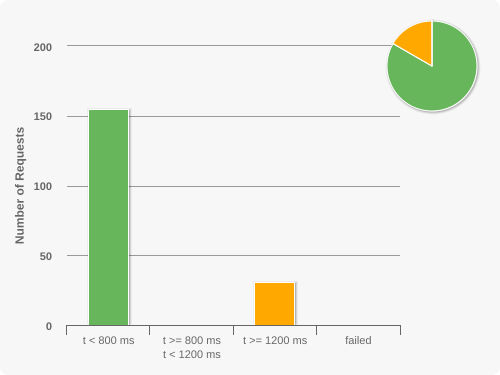
\includegraphics[width=0.5\linewidth]{figures/set}
    \caption{Response Times for Settings Simulation}
    \label{fig:resp_settings}
\end{figure}

\begin{figure}
    \centering
    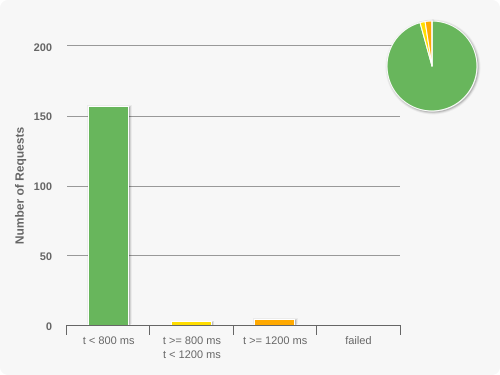
\includegraphics[width=0.5\linewidth]{figures/llm}
    \caption{Response Times for LLM-Model's Simulation}
    \label{fig:resp_llms}
\end{figure}

\begin{figure}
    \centering
    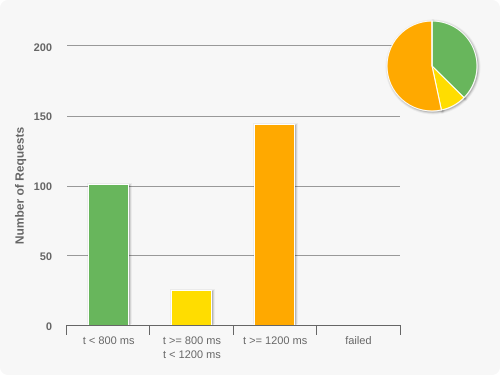
\includegraphics[width=0.5\linewidth]{figures/auth}
    \caption{Response Times for Authentication Simulation}
    \label{fig:resp_auth}
\end{figure}

\begin{figure}
    \centering
    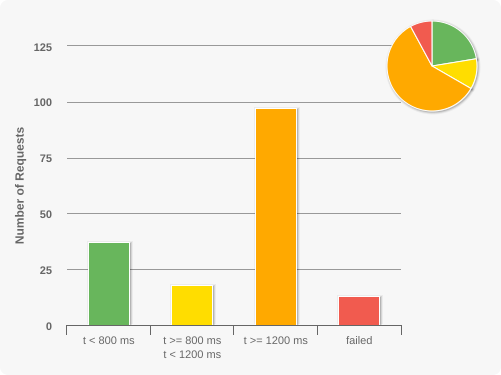
\includegraphics[width=0.5\linewidth]{figures/conv}
    \caption{Response Times for Conversation Simulation}
    \label{fig:resp_conv}
\end{figure}


\begin{figure}
    \centering
    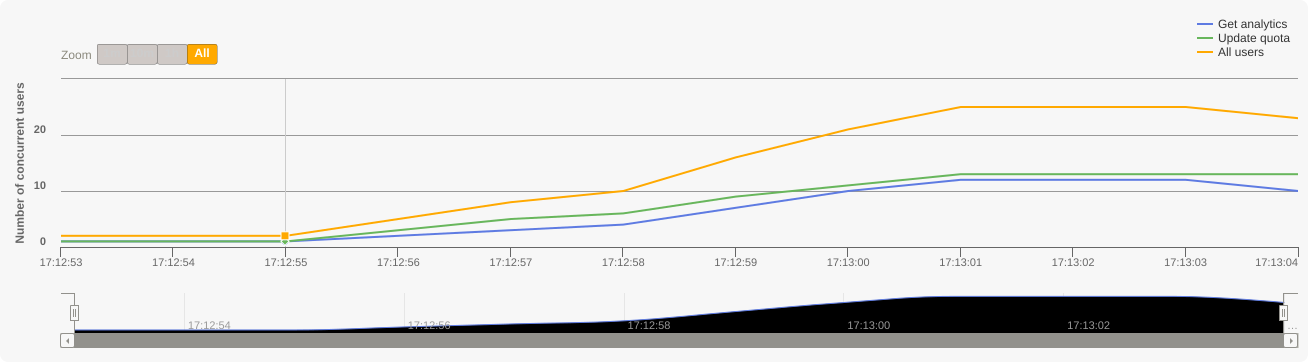
\includegraphics[angle=90,height=20cm]{figures/users}
    \caption{Total active users, Settings scenario}
    \label{fig:active-users}
\end{figure}

\begin{figure}
    \centering
    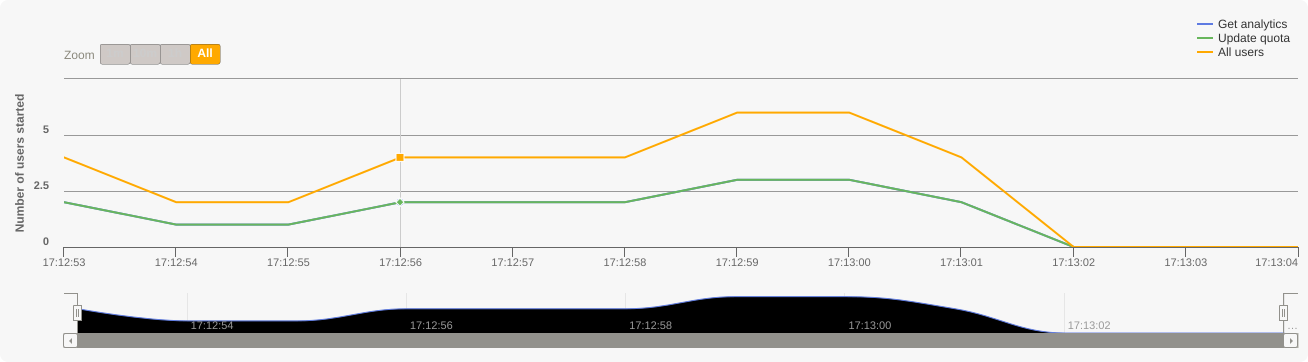
\includegraphics[angle=90,height=20cm]{figures/users_started}
    \caption{Total starting users, Settings scenario}
    \label{fig:active-users}
\end{figure}
%!TEX root = ../Pflichtenheft.tex

\chapter{Software Quality}

\section{Static Analysis}

To ensure a high level of code quality, static code analysis tools were used
for both the client and the server components of the system.

For the client, the TypeScript ecosystem was used. In particular,
\textit{TypeScript type checking} and \textit{ESLint} were applied to detect
potential errors early and to enforce a consistent coding style.
Additionally, the code was automatically formatted to ensure consistent
structure and readability.

For the server, static analysis tools were also used during development.
These tools help identify potential issues such as type inconsistencies,
unused variables, and possible runtime errors before execution.
Regular use of static analysis significantly contributed to maintaining
a high overall code quality throughout the development process.

\section{Extensibility}

The architecture of the system was designed to allow straightforward
extensibility. This is primarily achieved through the clear separation
of responsibilities within a layered architecture.

On the client side, the application follows a structured ViewModel
architecture in which presentation logic is separated from the
underlying business logic. New functionality can therefore often be
added by introducing additional ViewModels or services without
modifying existing components.

Similarly, the server follows a modular architecture. New functionality,
such as additional API endpoints or business logic modules, can be
implemented by adding new modules without affecting existing parts of
the system.

This clear architectural structure ensures that the system can be
extended with additional features in the future without requiring
major refactoring.

\section{Testability}

The system provides a high degree of testability due to the clear
separation between business logic and user interface components.

For the client, extensive automated unit tests were implemented using
the testing framework \textit{Vitest}. In total, 194 tests were executed,
all of which passed successfully. The achieved test coverage exceeds
95\% for statements, lines, and functions.

For the server, automated tests were implemented using the Python
testing framework \textit{pytest}. The test suite contains 142 tests,
all of which passed successfully during execution. The tests are
executed within a Python virtual environment and focus primarily on
the business and service layers of the application.

The server tests cover components such as:

\begin{itemize}
    \item API routes and service endpoints
    \item inference manager
    \item system manager
    \item user information manager
    \item prompt manager
    \item persistence repositories
\end{itemize}

A central test bootstrap was implemented in
\texttt{tests/conftest.py}. This configuration provides default
environment settings and lightweight dependency stubs, enabling the
test suite to run without requiring external services.

The current server test coverage is approximately 63\%. Core components
such as the service APIs, inference logic, system management, and
persistence layer are well covered by the tests. Lower coverage values
mainly originate from modules that depend on external integrations,
such as vector database initialization, graph generation internals,
OpenAI client transport logic, and validator subprocess paths.

During the development of the test suite, several improvements were
also made to the server implementation. These include fixing the
generation of JWT timestamps to use UTC-aware values and correcting
the initialization path for administrator profile pictures.

External dependencies such as network requests or browser APIs are
replaced with mock objects during testing, which allows the tests to
run independently of external services.

Some parts of the user interface, especially complex graphical
components, are not fully covered by automated tests, since they are
difficult to verify meaningfully with unit tests.

\section{Code Readability}

To improve code readability, particular attention was given to clear
structure and consistent naming of classes, methods, and variables.

Additional comments and documentation were added for central
components and complex logic areas. This improves the maintainability
of the code and makes it easier for future developers to understand
and extend the system.

By organizing the system into well-defined modules with clear
interfaces, the code remains understandable and manageable even as
the project grows.

\subsection{Measures to Improve Code Quality}

Several measures were implemented during development to further improve
the overall code quality.

One important step was the introduction of centralized structures for
commonly used configurations and error translations. This prevents
duplicate strings and inconsistent configuration definitions
throughout the codebase.

Furthermore, existing tests were extended and partially restructured
to increase test coverage and improve test stability. In particular,
mock objects were introduced for browser functionality and external
services so that tests can be executed independently from the runtime
environment.

These measures contribute significantly to the maintainability,
stability, and long-term extensibility of the system.
\chapter{Addressed Issues}
The following chapter presents issues that were found during the quality assurance phase.

\section{User Interface}\label{sec:user-interface}
Following issues were found in the user interface.
We also explain briefly how they were addressed and fixed.

\begin{itemize}
    \item \textbf{Unrecognizable Buttons or actions:} Changed label or icon
    \item \textbf{Incorrect message for username requirements:} Made error message more detailed
    \item \textbf{Visualization is lacking a legend:} Added different visualizations for different components
    \item \textbf{Visualization was hard to see in dark mode:} Changed color scheme
    \item \textbf{Prompt text is too small:} Increased font size
    \item \textbf{Chat search is case-sensitive:} Made case-insensitive
    \item \textbf{Misaligned button in signup window:} Made center-aligned
    \item \textbf{Missing information about model name:} Added info in the model-configuration window about llm-model provider naming
\end{itemize}

\subsection{Optional Improvements}
Following optional improvements were found:

\begin{itemize}
    \item Unnecessary sliders appear on some browsers
    \item Partial automatic navigation after some actions
\end{itemize}

\section{Client Internals}
Following issues were found in the internal client logic.
We also explain briefly how they were addressed and fixed.

\begin{itemize}
    \item \textbf{Send button is not working on some browsers:} Removed the \texttt{on} prefix from a custom event handler name
    \item \textbf{No way to manually change the UI language:} Added a toggle button
    \item \textbf{Wrong url destination after logout:} Made the client navigate to \textit{/login} after logout
    \item \textbf{Some users were not recognized to be authenticated by the auth guards:} Strictened the logic of the auth guards
    \item \textbf{Tokens were not saved locally:} Fixed the initialization logic of the token handler
    \item \textbf{Conversation screen would not react to navigations in some cases:} Forced a conversation reload when a navigation action is issued
    \item \textbf{Debug logs are visible on the browser console:} Removed debug print statements
\end{itemize}

\section{Server Internals}
Following issues were found in the internal server logic.
We also explain briefly how they were addressed and fixed.

\begin{itemize}
    \item \textbf{Context window given to the LLM was not always sufficient:} Changed the top-k parameter from 2 to 3
    \item \textbf{Timestamp in JWTs were dependant on the machines timezone:} Changed to now use UTC timestamps
    \item \textbf{File path for admin profile picture was hardcoded:} Admin profile picture is now according to the volume
     \item \textbf{Deleting an OpenAI model while an active chat existed caused the system to crash:} Added proper validation and handling when models are removed so existing chats fail gracefully instead of crashing the system
    \item \textbf{Email confirmation was not triggered when a user signed up without verifying their email and later authenticated via Google OAuth:} Adjusted the authentication flow so that OAuth login now correctly confirms the email address if it matches the account
    \item \textbf{Trash chunks were being inserted into ChromaDB:} Added a filtering step to detect and remove low-quality chunks before ingestion into ChromaDB.
\end{itemize}

%------Ende des Dokumentes------------------------------------------------------
\end{document}
